%pme2360
\section{Convecção Natural x Conveccção Forçada}
É muito semelhante ao que nós ja fizemos para convecção forçada.\\
Agente externo provocando o movimento do fluido: convecção forçada.
O que define convecção natural: transferência de calor devido a diferença
de temperatura.
Convecçao Mista: mistura das outras duas anteriores.
É possível calcular um numero de Nusselt que seja a soma das conveccoes 
natural e forçada.

% \begin{figure}[h]
% \begin{center}
% 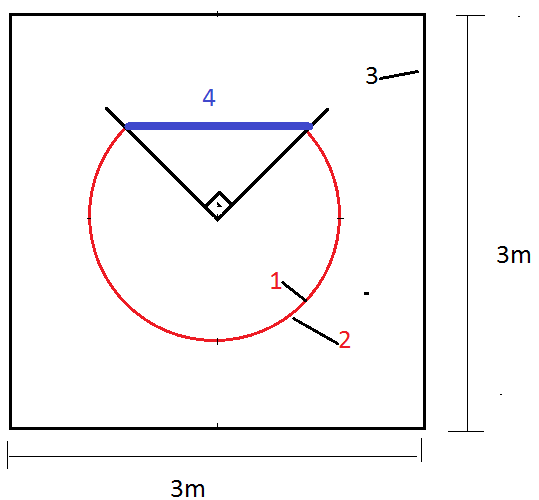
\includegraphics[scale=0.18]{./fig/1.png}
% \caption{\label{fig:1}1} 
% \end{center}
% \end{figure}

% \myfig[scale=.18]{figPME2360-20111026-01}{}

Se eu tenho um fluido quente embaixo e um fluido frio em cima formam-se correntes de convecção.

Em conveccçao forçada, os coeficientes nao dependiam da temperatura.
Agora, em convecção mista, também vão depender.

% \begin{figure}[h]
% \begin{center}
% 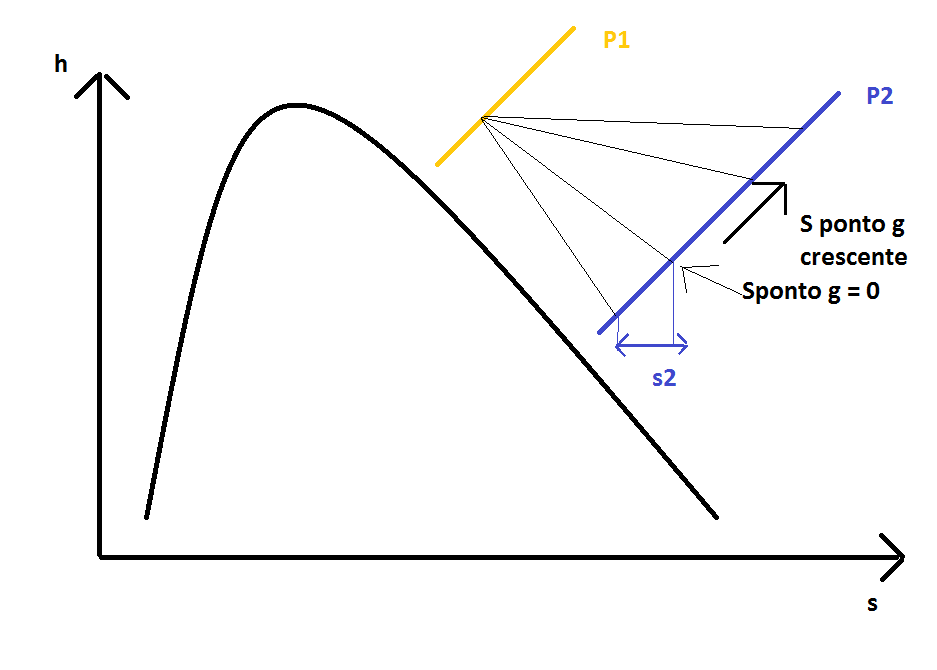
\includegraphics[scale=0.18]{./fig/2.png}
% \caption{\label{fig:2}2} 
% \end{center}
% \end{figure}

% \myfig[scale=.18]{figPME2360-20111026-02}{}

Quantidade de movimento na direçao x:
\begin{equation}
u\frac{du}{dx}+v\frac{du}{dy}=-\frac{1}{\rho}\frac{dp_{\infty}}{dx}-g+v\frac{d^{2}u}{dy^{2}}
\label{eq:1}
\end{equation}

Fora da camada limite:
\begin{equation}
\frac{dp_{\infty}}{dx}=-\rho_{\infty}g
\label{eq:2}
\end{equation}
\[\Delta \rho = \rho _{\infty}-\rho\]
Combinando as equações \ref{eq:1} e \ref{eq:2}
\begin{equation}
u\frac{du}{dx}+v\frac{du}{dy}=g\frac{\Delta \rho}{\rho}+v\frac{d^{2}u}{dy^{2}}
\label{eq:3}
\end{equation}

% \begin{figure}[h]
% \begin{center}
% 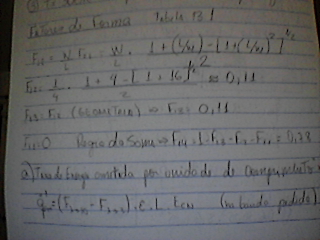
\includegraphics[scale=0.18]{./fig/3.png}
% \caption{\label{fig:3}3} 
% \end{center}
% \end{figure}

% \myfig[scale=.18]{figPME2360-20111026-03}{}

Coeficiente de expansão volumétrica:
\begin{equation}
\beta=-\frac{1}{\rho}(\frac{d\rho}{dt})=\footnote{aproximacao de Boussinesq} -\frac{1}{\rho}\frac{\rho _{\infty}-\rho}{T_{\infty}-T}
\end{equation}

\begin{equation}
\rho _{\infty}-\rho=-\rho\beta(T_{\infty}-T)
\label{eq:4}
\end{equation}

Combinando as equações \ref{eq:3} e \ref{eq:4}
\begin{equation}
u\frac{du}{dx}+v\frac{du}{dy}=g\frac{\beta (t_{S}-T_{\infty})}{u_{0}^{2}}T+\frac{1}{Re_{L}}\frac{d^{2}u}{dy^{2}}
\end{equation}

\newpage

\[u^{*}\frac{du^{*}}{dx^{*}}+v^{*}\frac{du^{*}}{dy^{*}}=g\frac{\beta (t_{S}-T_{\infty})}{u_{0}^{2}}T^{*}+\frac{1}{Re_{L}}\frac{d^{2}u^{*}}{dy^{*2}}
\]


\[u^{*}\frac{dT^{*}}{dx^{*}}+v^{*}\frac{dT^{*}}{dy^{*}}= \frac{1}{Re_{L}Pr}\frac{d^{2}T}{dy^{*2}}\]

\[u^{*}\frac{du^{*}}{dx^{*}}+v^{*}\frac{du^{*}}{dy^{*}}=\frac{Gr_{L}}{Re_{L}^{2}}T^{*}+\frac{1}{Re_{L}}\frac{d^{2}u^{*}}{dy^{*2}}
\]

\[u^{*}\frac{dT^{*}}{dx^{*}}+v^{*}\frac{dT^{*}}{dy^{*}}= \frac{1}{Re_{L}Pr}\frac{d^{2}T}{dy^{*2}}\]

Espera-se 
\[Nu_{L}=f(Re_{L},Gr_{L},Pr)\]

Condições de contorno:
\begin{itemize}
\item y = 0, u = v = 0, T=$T_{S}$
\item y$ \rightarrow \infty$, u $\rightarrow$0, T$\rightarrow T_{\infty}$
\end{itemize}

O que acontece quando você varia a espessura da camada limite? A variaçao da velocidade é menor com a maior espessura da camada limite (devido ao numero de Nusselt).

Parametro de similaridade:
\[\eta=\frac{y}{x}(\frac{Gr_{x}}{4})^{\frac{1}{3}} \]

\[f'''+3ff''-2(f')^{2}+T^{*}=0\]

\paragraph*{Exemplo} 
placa vertical com $T_{S}$ uniforme de 130º C e ar quiescente a 25º C. Determinar $\delta$ e $u_{max}$ para x=0.25 m

\[T_{f}=350K\]
\[Pr=0.7\]
\[Gr_{x}=6.718*10^{9}x^{3}\]
\[\nu = 20.92*10^{6}m^{2}/s\]
\[\eta = \frac{y}{x}(\frac{Gr_{x}}{4})^{1/4}=\frac{\delta}{0.25}(\frac{6.718*10^{9}*0.25^{3}}{4})^{1/4}=5\]

\[\delta = 1.746*10^{-3}m=17.5mm\]

\[u_{max}=0.47m/s\]
\[f'(n)=\frac{ux}{2\upsilon}Gr_{x}^{-1/2}=0.275\]

% \begin{figure}[h]
% \begin{center}
% 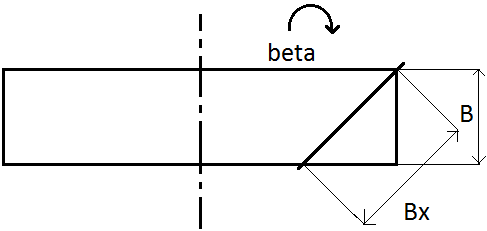
\includegraphics[scale=0.38]{./fig/4.png}
% \caption{\label{fig:4}4} 
% \end{center}
% \end{figure}

% \myfig[scale=.18]{figPME2360-20111026-04}{}

\[Nu_{x}=(\frac{Gr_{x}}{4})g(Pr)=(\frac{6.718*10^{9}*0.25^{3}}{4})*0.5=35.8\]
\[h=35.8*0.030/0.25=4.3W/m^{2}K\]
\[g(Pr)=\frac{0.75Pr^{1/2}}{(0.609+1.22Pr^{1/2})}\]

\[Ra_{x,c}=Gr_{x,c}Pr=6.718*10^{9}x^{3}*0.7\]